\section{Efectul Compton}

Atunci când un fascicul de raze X, provenit de la o sursă $S$, trece printr-un
bloc de grafit $G$, radiațiile incidente sunt împrăștiate în toate direcțiile.

\begin{wrapfigure}[9]{r}{0.5\textwidth}
    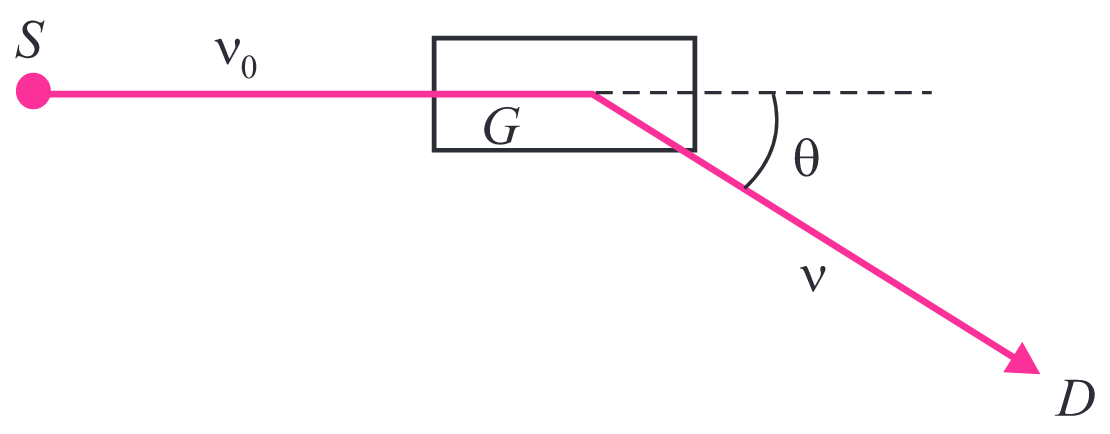
\includegraphics[width=0.5\textwidth]{fig/compton}
    \caption{Experimentul Compton, reprezentat schematic}
\end{wrapfigure}

Pentru diferite unghiuri de împrăștiere $\theta$, detectorul $D$ înregistrează,
pe lângă radiația incidentă cu lungimea de undă $\lambda_0$, și o altă radiație
cu lungimea de undă \( \lambda > \lambda_0 \).

Din punct de vedere macroscopic, lumina, și în general radiația electromagnetică,
este o undă. Din punct de vedere microscopic, lumina este un ansamblu de particule
cuantice.

\parbreak

Fenomenul, observabil pentru lungimi de undă mici, ca în cazul razelor X și
\gamma, deci pentru frecvențe mari (\(\lambda = \frac{c}{\nu} \)), a fost
explicat de către Compton pe baza naturii corpusculare a undelor electromagnetice,
adică prin existența fotonilor.

\emph{%
    Efectul Compton este fenomenul de împrăștiere elastică a fotonilor pe
    electronii liberi, în urma căreia, pe lângă radiația incidentă, apare și
    o radiație cu lungimea de undă mai mare (frecvența mai mică).
}

În cazul în care atomii substanței pe care se produce împrăștierea sunt ușori,
ca în cazul atomilor de siliciu, bor sau bariu, atunci energia de legătură a
electronilor de valență este mult mai mică decât energia fotonului incident
$h\nu_0$, iar electronul poate fi considerat practic liber.

Indiferent de natura substanței pe care se produce împrăștierea, diferența
\( \lambda - \lambda_0 \) este direct proporțională cu \theta, relația dintre
ele fiind:
\[ \lambda - \lambda_0 = a(1 - \cos\theta) \]
unde \( a = 2,423 \cdot 10^{-3} ~ \mathrm{nm} \).

\begin{wrapfigure}{r}{0.4\textwidth}
    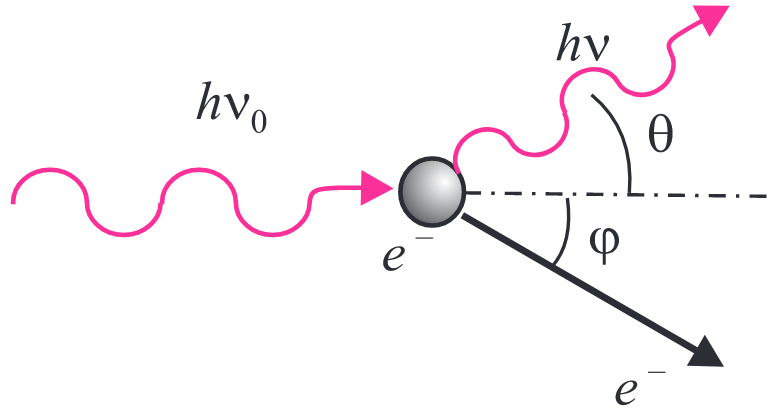
\includegraphics[width=0.4\textwidth]{fig/compton_electron}
    \caption{Fotonul împrăștiat și electronul de recul în efectul Compton}
\end{wrapfigure}

Dacă electronul substanței împrăștietoare se afla în repaus înainte de
interacțiunea cu fotonul (fig. 9), legea conservării energiei este:
\[ h\nu_0 = h\nu + E_c + L \]
unde $h\nu_0$ și $h\nu$ sunt energiile fotonilor cu lungimea de undă \lambda,
respectiv $\lambda_0$, $E_c$ este energia cinetică a electronului de recul,
iar $L$ este lucrul mecanic de ieșire a electronului din atomul substanței.

Electronul fiind liber, putem neglija $L$.

Această interacțiune dintre foton și electronul liber poate fi tratată ca o
ciocnire elastică, aplicându-se legile conservării energiei și impulsului.

Având o masă foarte mică, electronul atinge viteze mari. Prin urmare, legile
conservării energiei și impulsului se scriu relativist:
\begin{equation}
    h\nu_0 + m_0c^2 = h\nu + mc^2
\end{equation}
\[ \vec{p_0} = \vec{p}+ \vec{p_e} \]

Proiectând relația a doua pe $Ox$ și $Oy$, și știind că \( p_0 = \frac{h\nu_0}{c}, p = \frac{h\nu}{c}, p_e = mv \), obținem:
\begin{flalign*}
    &\text{pe $Ox$:} &p_0 &= p\cos\theta + p_e\cos\alpha
    &\Leftrightarrow& &\frac{h\nu_0}{c} &= \frac{h\nu}{c}\cos\theta + mv\cos\alpha &\\
    &\text{pe $Ox$:} &0 &= p\sin\theta - p_e\sin\alpha
    &\Leftrightarrow& &0 &= \frac{h\nu}{c}\sin\theta - mv\sin\alpha &
\end{flalign*}

Rezultă că:
\[
    mv\cos\alpha = \frac{h\nu_0}{c} - \frac{h\nu}{c}\cos\theta
    \qquad\qquad\qquad
    mv\sin\alpha = \frac{h\nu}{c} \sin\theta
\]

Ridicăm la pătrat și adunăm, obținând:
\begin{equation}
    m^2v^2c^2 = h^2 (\nu_0^2 + \nu^2 - 2\nu_0\nu\cos\theta)
\end{equation}

Scriem relația (1) sub forma
\( mc^2 = h(\nu_0 - \nu) + m_0c^2 \)
și o ridicăm la pătrat:
\begin{align*}
    m^2c^4 &= [h(\nu_0 - \nu) + m_0c^2]^2 \\
           &= h^2(\nu_0^2 - 2\nu_0\nu + \nu^2) + 2m_0c^2h(\nu_0 - \nu) + m_0^2c^4
\end{align*}

Din această relație scădem (2), și rezultă:
\begin{equation}
    m^4c^4 \left(1 - \frac{v^2}{c^2}\right)
    = -2\nu_0\nu h^2(1 - \cos\theta) + m_0^2c^4 + 2m_0c^2h(\nu_0 - \nu)
\end{equation}

Cum \( m = \frac{m_0}{\lorentzradical} \), relația (3) devine:
\begin{align*}
    \nu_0\nu h(1 - \cos\theta) &= m_0c^2 (\nu_0 - \nu) \\
    1 - \cos\theta &= \frac{m_0c^2}{h} \left(\frac{1}{\nu} - \frac{1}{\nu_0}\right)
    = \frac{m_0c}{h}(\lambda - \lambda_0)
\end{align*}

Rezultă:
\[ \Delta\lambda = \frac{h}{m_0c}(1 - \cos\theta) \]

Mărimea \( \Lambda = \frac{h}{m_0c} \) este lungimea de undă Compton, și are
valoarea \( \Lambda = 2,427 ~ \mathrm{pm} \) atunci când particula cu care
interacționează fotonul este un electron cu masa
\( 9,1 \cdot 10^{-31} ~ \mathrm{kg} \),
\( h = 6,626 \cdot 10^{-34} ~ \mathrm{J \cdot s} \),
și \( c = 3\cdot10^8 ~ \mathrm{m/s} \).

În concluzie, diferența lungimilor de undă a celor două radiații este:
\[ \Delta\lambda = \Lambda(1 - \cos\theta) = 2\Lambda\sin^2\frac{\theta}{2} \]

În cazul particulelor ce au masa mai mare decât masa electronului, $\Lambda$ ia valori
foarte mici, de regulă neglijabile față de lungimea de undă a radiației incidente.
